\newpage

\section{Anechoic Chamber measurements}

\subsection{Purpose}

The purpose of this experiment is to test our sound localization algorithms in a controlled environment. An experiment is set up in the Anechoic chamber where a tetrahedral array receives sound waves emitted by a point source. The source position is fixed and the microphone array is rotated aorund its axis in order to change the receiving angle of the wave. A diagram of the experiment is displayed in figure \ref{fig:Anechoic1} where the two test configurations are shown: 0 and 30 degree.  The source is chosen to be a pink noise as in our simulation but recording of a 300Hz sinusoïd are performed to check the delay between the microphones. In order to recreate the far field condition in the limited space of the anechoic chamber the array is placed as further away from the source and the array aperture is reduced in order to reduce the size of the array and obtain a better plane wave propagation. 

\subsection{Diagram and pictures}



\begin{figure}[H]
    \centering
    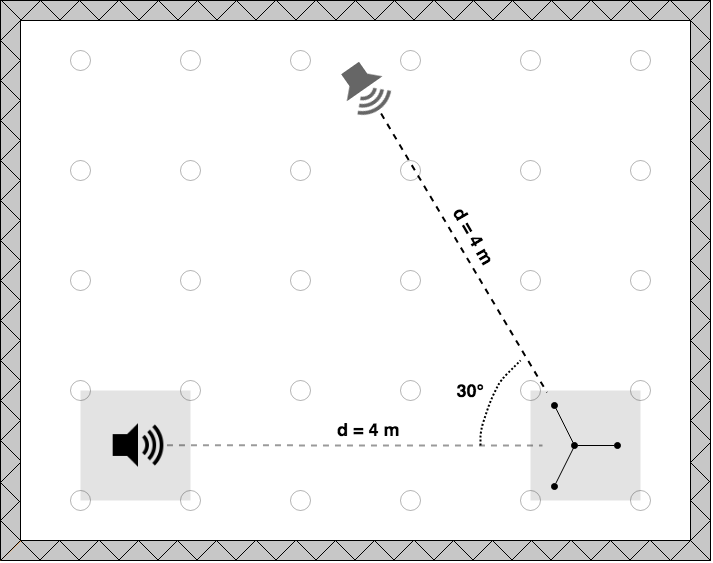
\includegraphics[width=0.9\textwidth]{Figures/Anechoic1.png}
    \caption{Diagram of the experiment}
    \label{fig:Anechoic1}
\end{figure}
 
 
 
 


\subsection{Stimuli and settings}

The point source is emitted by a Brüel \& Kjær omnisource type 4296 with operating frequency of 100 to 5000 Hz. The Brüel \& Kjær PULSE system is used to record the sound picked up by the microphone array and the operating frequency of the system is 131072 Hz which is the highest sampling frequency available on the system. The prototype microphone array allows to adjust the aperture size from 0,1m to 1m. As discussed earlier the aperture is reduced to 0,395m. Assuming that strong periodicity exist in the signal, the array could in theory work with waves of frequency up to 874 Hz before aliasing occurs. In our case where there is no strong periodicity, we distinguish noise with much higher frequency \ref{REF}

\begin{equation}
    f=\frac{c}{\lambda}=\frac{345}{0,395} \approx 874 (Hz)
\end{equation}



 
 
 \subsection{Delay between the microphones}
 
 In order to know the accuracy of the measurements, sample delay is measured at a single frequency. In order to avoid the pressure field frequency zone of the anechoic chamber and array aliasing,  a sin wave of 300 Hz is choosen. A single frequency is chosen therefore this measurement is representative for the group delay at this representative frequency. 
 
 
 \begin{figure}[H]
    \centering
    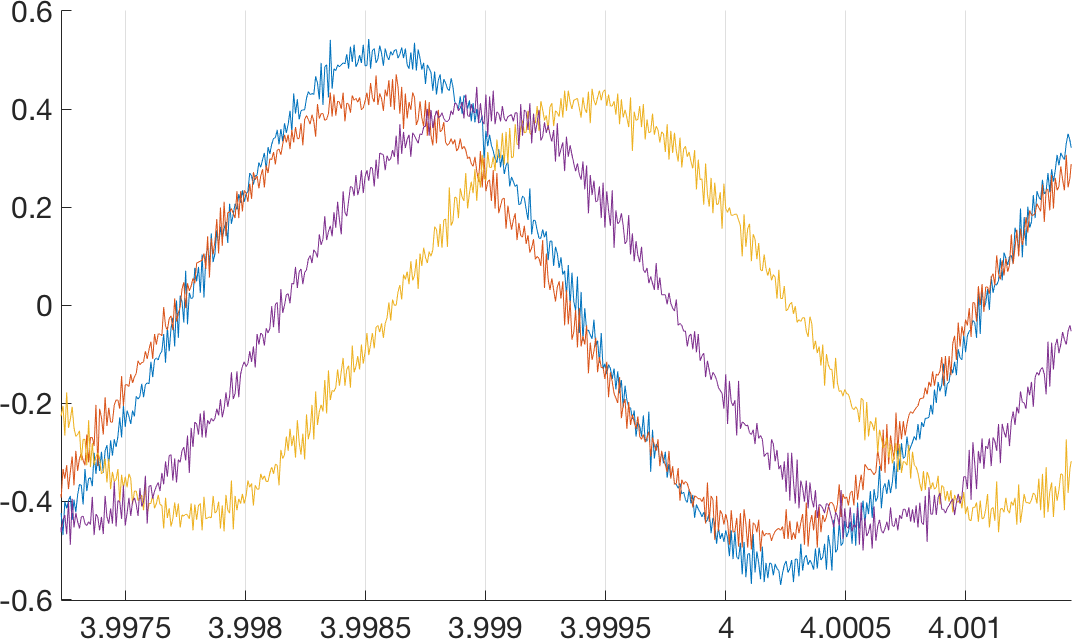
\includegraphics[width=0.8\textwidth]{Figures/delaytetra300Hz.png}
    \caption{sin wave recorded by the four microphones.}
    \label{fig:pinknoise}
\end{figure}
 
 
\begin{center}
  \begin{tabular}{ | l | c | r | r | r |}
    \hline
    Delays & Mic 1 & Mic 2 & Mic 3 & Mic 4 \\ \hline
    Mic 1 & X & -6&114 & 52  \\ \hline
    Mic 2 &   & X &120 & 58  \\ \hline
    Mic 3 &   &   & X  &-61  \\ \hline
    Mic 4 &   &   &    & X   \\ \hline
  \end{tabular}
  \captionof{table}{Sample delay measured between the microphones at 0 incidence}
\end{center}
 


\begin{figure}[H]
    \centering
    \begin{subfigure}[t]{0.5\textwidth}
    \centering
    \includegraphics[width=0.9\textwidth]{Figures/IMG_7337.png}
    \caption{B\&K Omnisource}
    \label{fig:Omnisource}
\end{subfigure}%
\begin{subfigure}[t]{0.5\textwidth}
        \centering
    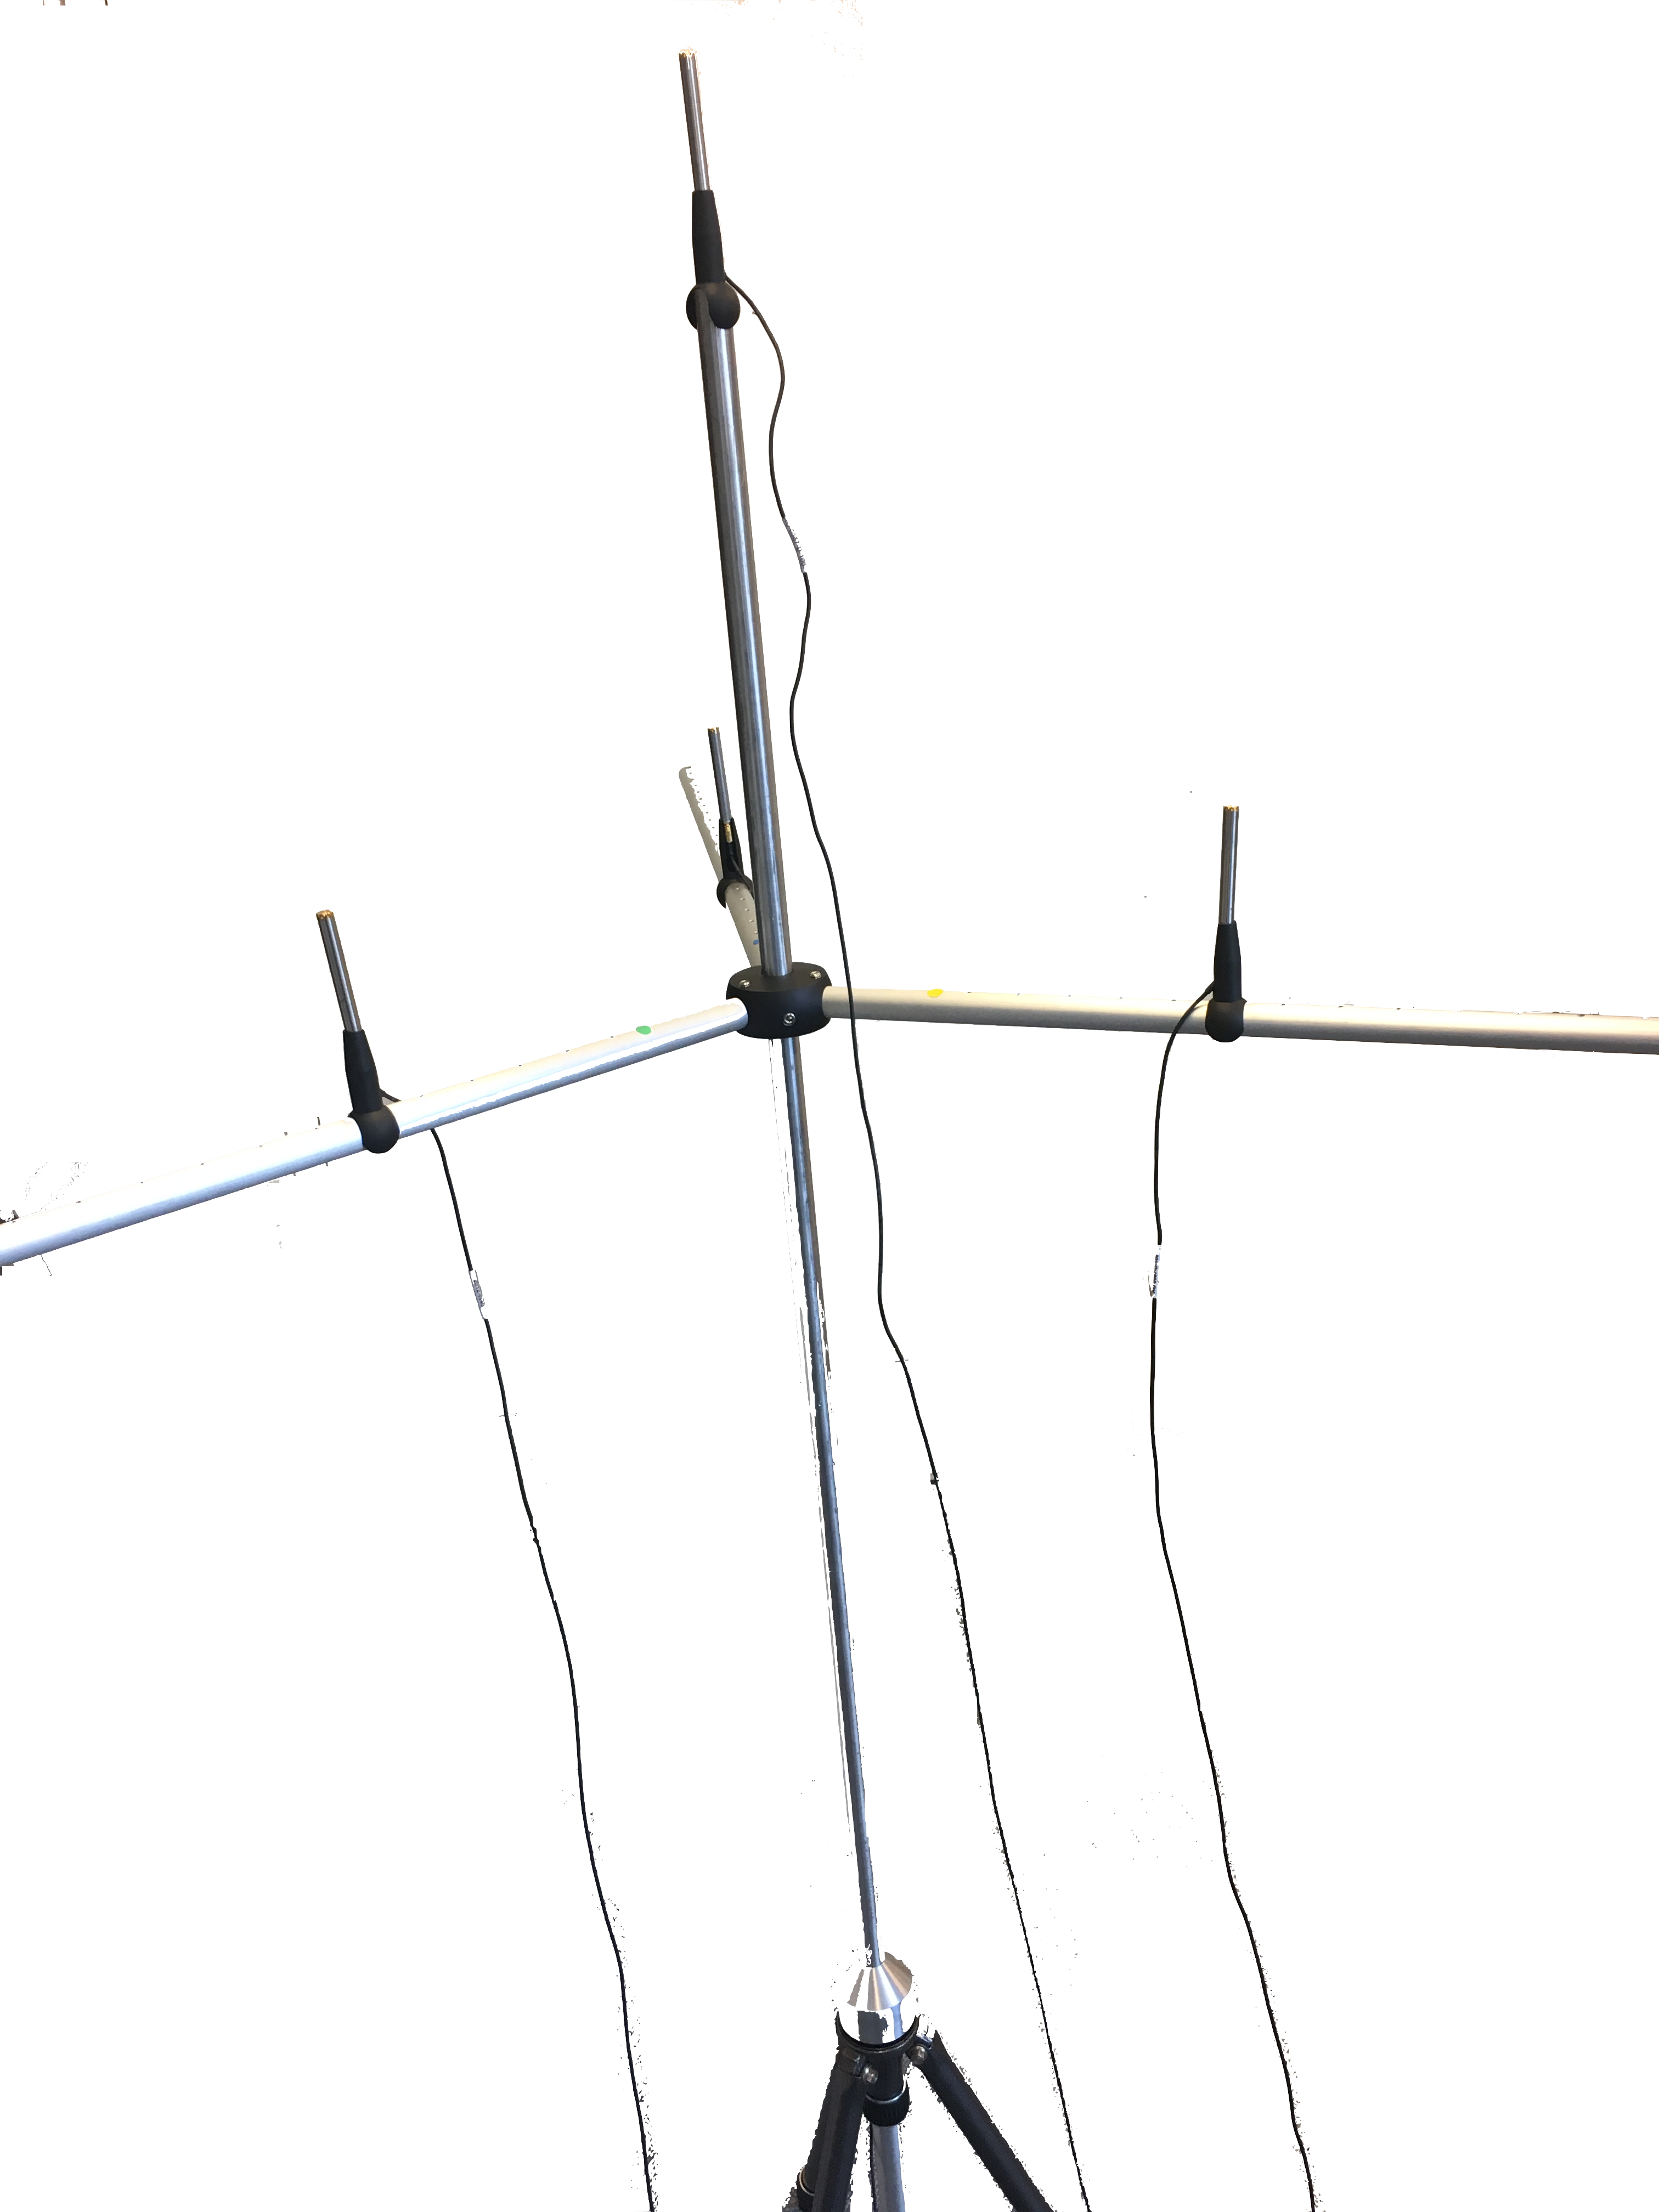
\includegraphics[width=0.9\textwidth]{Figures/Arraymicrophone.png}
    \caption{Prototyped microphone array}
    \label{fig:Array}
\end{subfigure}
\end{figure} 



\subsection{AAU number List}



\begin{figure}[H]
    \centering
    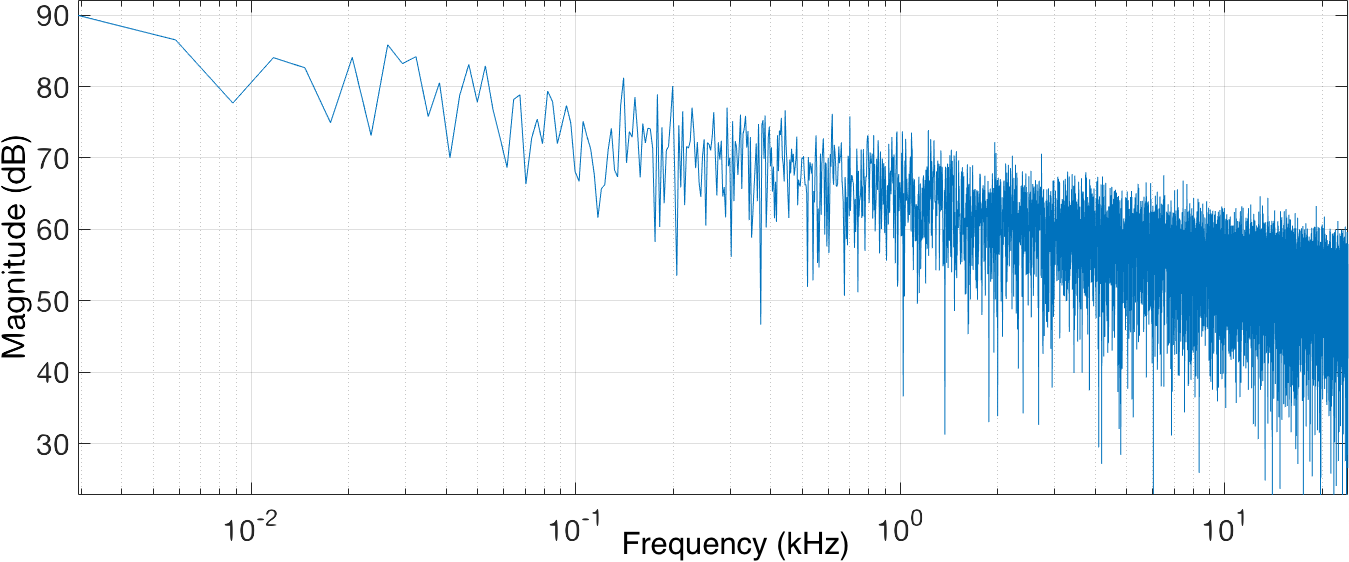
\includegraphics[width=1\textwidth]{Figures/pinknoise.png}
    \caption{Source stimuli}
    \label{fig:pinknoise}
\end{figure}
 